\chapter{Background of Trans-Himalayan Languages}

\section{Introduction}
The \lfam\ family, also referred to as Tibeto-Burman or Sino-Tibetan, is a primary language family spoken throughout parts of Eastern Asia, centering on the Himalayas and extending to the east, through Myanmar and the Shan Hills. Languages of this family are also spoken throughout China, both historically and as the official language of China, Standard Mandarin (\textit{pǔtōnghuà}). Their overall geographic distribution is shown in \mapref{fig:OverallMap}, showing the family stretching as far north as Northern China (Mandarin, Sinitic), to the western reaches of the Himalayan range in Kashmir in the west (Purik, Tibetic). In the south, the Karen subfamily stretches south towards the Malay Peninsula, and in the east, more recent migrations have brought Sinitic Languages to Taiwan. The family includes major languages such as Mandarin and Cantonese, both in the Sinitic branch, Burmese, in the Ngwi-Burmese branch, and Tibetan, in the Bodish branch. The remainder of the languages in the family are, for the most part, spoken by smaller indigenous communities throughout the region. Glottolog reports almost 500 languages in the family \cite{glottolog}, while \citeA{Owen-SmithHill2013} report around 600, with over 1.4 billion total speakers \cite{ZhangH2020Baye}, approximately 900 million of which are native Mandarin speakers \cite{Ethnologue}. While the majority of the family's speakers exist to the North of the Himalayan range in China, this statistic is a result of the overwhelmingly large number of speakers of Sinitic languages, specifically Mandarin and its dialects. The greatest area of linguistic diversity, on the other hand, falls to the South, in the Eastern Himalaya region covering Eastern Bhutan and far North-Eastern India \cite{BlenchPost2013}.

This chapter comprises an overview of the history of research into the \lfam\ family, both in the Western tradition and otherwise, a major part of which is the growing body of grammatical description that provides a foundation for this project. It also provides an overview of some contemporary ongoing discussions in the field, and establishes the stance taken in this project with regards to these disagreements. Lastly, it discusses the work that has been undertaken in the historical domain, looking both at surviving primary sources of historical languages, as well as the current extent of reconstructions of proto-languages.

\begin{map}
\centering
\includegraphics[width=\textwidth]{FullExtent.png}
\caption{The approximate full extent of the \lfam\ languages, missing some parts of the People's Republic of China, and of Taiwan. There are areas inside this extent where \lfam\ languages are not spoken, or where non-Trans-Himalayan languages are spoken (e.g. Kra-Dai, Austroasiatic, Mon-Khmer, Indo-European).}
\label{fig:OverallMap}
\end{map}


\section{History of Research into \lfam\ Languages}\label{s:historyofresearch}
Linguistic research is no new innovation in the Himalayas and Eastern Asian. Scholars have written about language and its history and use well before the arrival of any Western Academic Tradition to the region. Literary traditions have existed in a number of regions for many centuries, and much of this literature informs contemporary linguistic research.

Old and Middle Chinese Rime Books, books grouping characters by their pronunciations, have been widely used as sources informing contemporary reconstructions of the languages \cite{Baxter1992}. The books were composed as early as the 2nd Century CE, through to the 9th. Due to the (generally) non-phonetic nature of the Chinese writing system, these books were compiled to create some record or method of instruction into the pronunciation of each character, by sorting each character in terms of its onset and rime \cite{Ji2021}.

There is similarly a very longstanding tradition of linguistic research in Tibet. Perhaps the most important of these are the \texttibetan{སུམ་ཅུ་པ} \textit{Sum cu pa} and \texttibetan{རྟགས་ཀྱི་འཇུག་པ} \textit{rTags kyi 'jug pa}, both attributed to 7th century scholar Thönmi Sambhoṭa, who is also credited with the development of the Tibetan writing system \cite{MuellerWitter2009}. These treatises comprise early grammatical descriptions of the language at the time, and are, at least according to legend, the only two survivors of a corpus of eight written by Thönmi Sambhoṭa \cite{Miller1963}, and are accompanied by a tradition of more recent of commentaries and translations \cite{Chashab2008}. There have been questions raised as to whether or not the attribution of these works to Thönmi Sambhoṭa is historically accurate, both for the grammatical treatises and development of the script. Arguments have been made that the treatises could have been written several hundred years later than legend reports \cite{Miller1963}. Aside from various historical inconsistencies or points of uncertainty when dealing with primary sources, \citeA{Miller1963} notes that the \textit{Sum cu pa} and \textit{rTags kyi 'jug pa} alone cover both the syntax and morphology of the language respectively \cite{Chashab2008}, leaving the question of what the other six treatises would have actually addressed. There seems to have been little reference in the Tibetan tradition as to the contents of this lost body of work, suggesting that they may never have existed.

While it is important to note this history of research and grammatical description in China and Tibet, there is little evidence of grammaticalised epistemic marking in Old Tibetan, in that the modern evidential-egophoric paradigm had not yet developed \cite{Hill2014} (though some distinctions have been described for Middle Classical Tibetan \cite{Oisel2024}). Similarly, it does not appear that any relevant grammatical phenomena were present in Old Chinese (which is, at least at this stage, similarly the case for the modern Sinitic languages), with the exception of adverbs marking epistemic modality\footnote{There is a question surrounding the definition of an adverb versus a particle (that is, lexical versus grammatical) that I will not attempt to answer in this chapter.} \cite{Pulleyblank1995}. As such, this early research provides no extra data for analysis. That said, it does mean, at least in the case of Modern Tibetan, the evidential-egophoric system is an innovation or areal borrowing, rather than a system that might have been inherited from any proto-language. Further historical languages with surviving records but lacking contemporaneous linguistic research are presented in Section \ref{s:AncientLiteraryLanguages}.

In contrast to this centuries-old body of research into Tibetan and Chinese grammar and phonology, the history of Western research and interest into the family is only some 200 years old. A `Tibeto-Burman' language family containing Chinese, Tibetan, and Burmese, and excluding geographically close language groups such as Kradai, Austroasiatic was first proposed by Julius von Klaproth in 1823 \cite{VanDriem2014}, though this was by no means a widely accepted theory until much later. Much of the other earliest research into the language family by Western Scholars was built on racist ideas of language structure, equating the lack of inflection in group such as the Sinitic and Tai languages were a result of a lack of mental capacity \cite{VanDriem2014}. Comparative evidence of a link between Tibetan and Chinese was not found, however, until the early to mid 20th Century, with the work of Robert Schafer, first published in 1939. This work, however, still included the Tai languages in the Phylum, a clade which would not be readily dropped from the family until much later \cite{Matisoff1991}. \citeA{Handel2008} reports another source around the same period, a 1937 survey of the languages and dialects of China by Li Fang-Kuei, that also included neighbouring families such as Tai and Miao-Yao, which is noted in the editorial of its 1973 republication to have been an influential piece of literature in the area of study through the mid 20th Century \cite{Li1973}.

The past few decades have seen a rapid increase in the amount of research on the \lfam\ family in the Western Academic Tradition, though research has been conducted to some extent since the early 19th Century \cite{VanDriem2014}. In 1991, \citeA{Matisoff1991} suggested that the field was no older than 50 years, and had only seen substantial growth since the late 1960s. This recent growth in research can be seen in \figref{fig:PublicationsChart}, which shows the number of publications on \lfam\ linguistics by year, as indexed by the Glottolog database \cite{glottolog}. The drop-off in the most recent years can in part be attributed to the fact that 2021 is not yet over, and that more recent publications have likely not yet been entered into the database. The rise that can be seen starting in 1950 and accellerating substantially over the past 20 years can be attributed to a number of factors. The past few decades have seen an increase in the accessibility of many of these areas, physically and legally. Many of the states in North Eastern India only opened to international researchers within the past decade, allowing a substantial increase in research output focused on this region \cite{BlenchPost2013}. A similar situation can be seen in Bhutan, where research access has historically, and even to the present, been severely restricted (Hyslop, p.c.). It is no coincidence then that many of the subfamilies with very limited description are in this region (e.g., Gongduk, Lhokpu in Bhutan (see Section \ref{ss:THOverview:Subfamilies}), Digarish, Mudzuish in North-Eastern India.) This uneven descriptive coverage and its implications for this project are further discussed in Sections \ref{ss:THOverview:HighLevelStructure} and \ref{ss:THOverview:Subfamilies}.



\begin{figure}

\centering
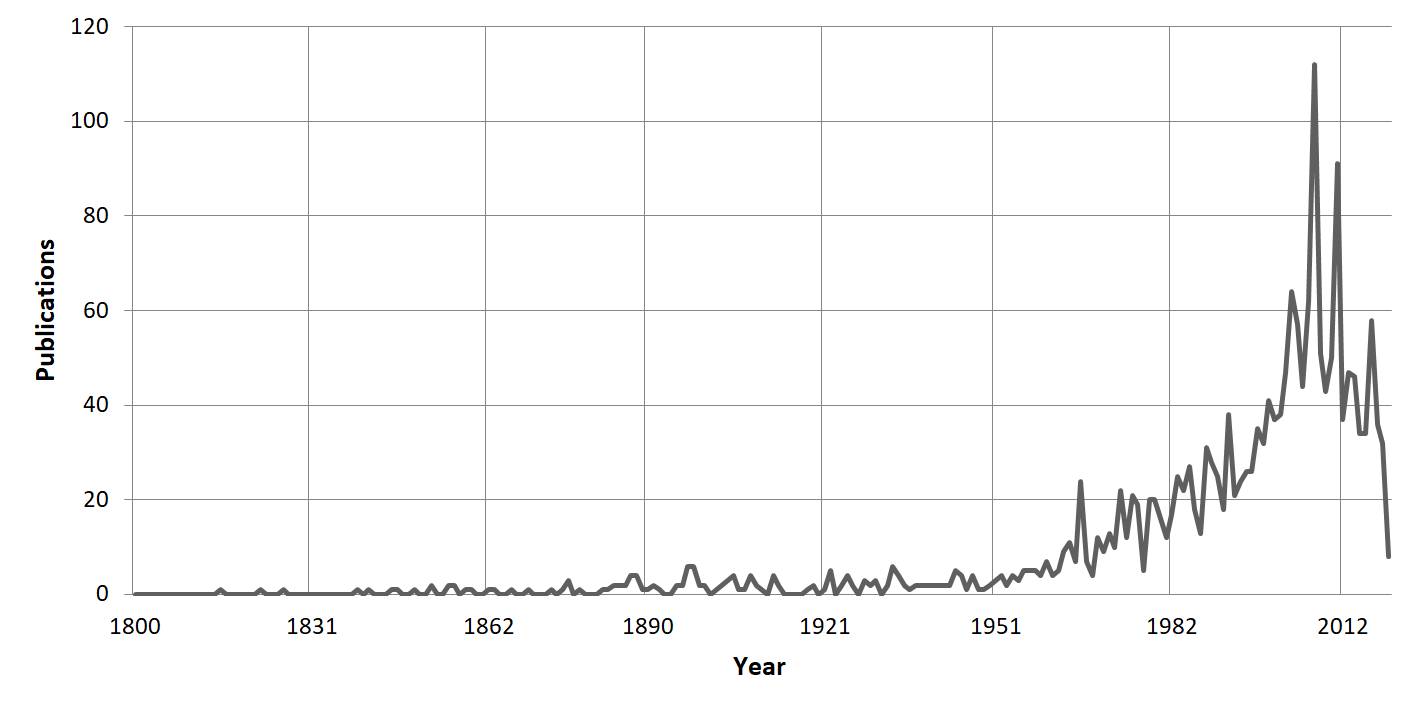
\includegraphics[width=\textwidth]{PublicationsChart.png}
\caption{Number of publications on the \lfam\ family recorded in the Glottolog database by year \cite{glottolog}}
\label{fig:PublicationsChart}
\end{figure}




\subsection{Dialects or Languages?}\label{s:DialectsorLanguages}
The question of the distinction between a language and a dialect is, of course, all pervasive to linguistics. Different interpretations of this distinction in different research traditions and political systems in the region have created an imbalance in the definition of languages and dialects in the family. \citeA{LaPolla2016} suggests that languages predominantly researched by linguists in the Chinese academic sphere, especially in the Sinitic branch, tend to more commonly be considered dialects of single broader languages, while languages researched by other linguistics, namely in the Indian academic sphere, tend to be considered separate languages in a more closely related subfamily.

This is also reflected at a policy level, in terms of how governments identify and classify various ethnolinguistic groups. \citeA{Bradley2002} give an extreme example from the Eastern Indo-Chinese border, where India officially identifies over 50 different `scheduled tribes' or ethnic groups, which are all grouped into a single Luoba `nationality' across the border by China.

While these two tendencies don't necessarily produce differing results in terms of isolated descriptions (descriptions of separate `dialects' of languages spoken in China have been conducted similar to descriptions of separate `languages' spoken elsewhere \cites{Lai2017}{TaylorAdams2020}), it can cause skew at a typological level, as there is a possibility that similarly divergent groups of `languages' or `dialects' will be identified as its own subfamily if spoken in India, but not in China. This has been raised as a potential criticism of \citeA{VanDriem2014} \cite{LaPolla2016}, and presents a potential issue in sampling for this project. That is, will a region of high linguistic diversity be missed or underrepresented as it is classified in such as way that seems to (deliberately or otherwise) minimise recognition of this diversity?


\section{Current Opinions in the Literature}
\subsection{Situating the Sinitic Branch in the Family}\label{ss:THOverview:HighLevelStructure}

Current opinion on the structure of the family in the literature is strongly divided, into two main schools of thought, predominantly centred on the highest-level division in the family genealogically. One school of thought suggests that the family is divided into two primary branches: `Sinitic' and `Tibeto-Burman'. Alternatively, some scholars argue that this binary division is incorrect, and that the Sinitic subfamily exists at a lower level within the overall family. These two mutually exclusive hypotheses will be henceforth referred to as the Sinitic-Divergent and Other-Divergent hypotheses.

A number of recent studies have found evidence in favour of the Sinitic-Divergent hypothesis through computational methodologies \cites{ZhangM2019Baye}{ZhangH2020Baye}{Sagart2019Baye}, namely Bayesian analyses and methodologies from fields of genetics, using cognate sets as an equivalent to genetic markers. While these three papers are able to agree on their support of the Sinitic-Divergent hypothesis, they otherwise disagree on the internal structure of the Tibeto-Burman branch and the time-scale of the family as a whole. \citeA{Sagart2019Baye} report an origin around 7,400 years BP, with a millet-farming origin, or urheimat, in North-Eastern China. \citeA{ZhangM2019Baye} on the other hand reports a slightly earlier mean age (about 5,800BP) and an urheimat much further south-west, in the eastern reaches of the Tibetan Plateau. Finally,  \citeA{ZhangH2020Baye} suggest an even earlier origin, at 8,000 years BP, and while not providing a clear urheimat, they do suggest that the Sinitic/Tibero-Burman division occurred prior to the development of widespread agriculture in China.

A number of potential issues in these methodologies have been identified by various researchers. \citeA{ZhangH2020Baye} themselves highlight some methodological concerns in \citesA{ZhangM2019Baye}{Sagart2019Baye}, namely surrounding the representativeness of their datasets. They suggest that their dataset presents a more evenly distributed cross-section of the language family by subfamily, with a lower standard deviation in percentage of languages in each subfamily sampled \cite{ZhangH2020Baye}. They also note that \citeA{Sagart2019Baye} contains no data at all from the Karenic or Naga subfamilies, with Karenic languages being spoken geographically much further south than other languages in the family.

This criticism, however, can extend to any study aiming to computationally analyse high level structures of any language family. That is, if a dataset is missing particularly linguistically or geographically divergent data, it is difficult to see it as an accurate representation of the data. Similarly, if data from only one language from a given sub-family is included, but many languages from another, that dataset might be similarly skewed. \citeA{ZhangH2020Baye} notes this as an issue in \citesA{ZhangM2019Baye}{Sagart2019Baye}, and reports an a more even coverage of each subfamily than in the two previous studies. However, this relies on the subfamilies as given in the paper being representative of the actual subfamilies that exist from a historical perspective. There is a degree of a circular logic here. In order to create an even sample of the language family by subfamily, one needs first to know what these subfamilies actually are, which is in many ways exactly what these studies are trying to discover.

\citeA{ZhangH2020Baye} also only report subfamily coverage for a small set of subfamilies, grouping a large number of other languages into the category ``isolates'' and as such ignoring any subfamily relations they may have. In some cases, such as with Tujia or Meithei, this agrees with other literature such as \citeA{VanDriem2014}, though in other cases it seems to fail to consider the language's other close relations. For instance, Kinnauri is listed as an isolate in the list of languages, despite being classified in a separate West Himalayish subfamily by both \citesA{VanDriem2014}{Thurgood2017STIntro}, a subfamily with, in addition to Kinnauri, at least 14 other languages \cite{glottolog}. A similar issue exists with the Kachinic languages, which are represented solely by the so-called `isolate' Jingpo (at the exclusion of 8 other languages), as well as with the rGyalrongic languages, which are represented by Jiarung, Daofu Horpa, and Ergong, all of which are given as isolates despite being grouped together in wider literature \cites{Honkasalo2019}{Gates2021}\footnote{A pervasive challenge in research on the \lfam\ family is the lack of agreement on language names. `Jiarung' most likely refers to the rGyalrongic languages here, though the core group of the subfamily is varyingly referred to as a group of languages or dialects of a single language. See Section \ref{s:DialectsorLanguages} for further discussion.}.

\subsection{Name of the Family}

This uncertainty surrounding the high level internal structure of the language family also has implications for the name of family itself, in that the historically most widespread name `Sino-Tibetan' specifically references the Sinitic-Divergent hypothesis. A number of alternatives to this have been suggested, either to actively reject the Sinitic-Divergent hypothesis or to remain agnostic. `Tibeto-Burman' has been used fairly widely as an alternative name for the family as a whole, in contrast to Tibeto-Burman as the non-Sinitic branch of a Sinitic-Divergent Sino-Tibetan family \cite{VanDriem2007}. While this no longer supports a Sinitic-Divergent structure for the family, it also seems to suggest some level of primacy or greater importance to Tibetan and Burmese languages, one of the very issues initially identified with the term Sino-Tibetan. A second alternative, `Trans-Himalayan', has been more recently suggested, avoiding reference to any specific language to avoid any such suggestions of internal structure or greater importance in certain languages or subfamilies \cite{BlenchPost2013}. Here, `Trans-Himalayan' refers to the geographic distribution of languages in the family across entire Himalayan range, and well to the North and South. A potential point of confusion with this name is the inconsistency in meaning between this term and the use of `trans' in wider toponomy. For example, `Transalpine' traditionally refers not to the area across \textit{both} sides of the Alps, but on the \textit{other} side (from Rome), and is contrasted with `Cisalpine' (on \textit{this} side of the Alps).

The term \lfam\ is used in this thesis \lfamreason\

\subsection{Overview of Subfamilies}\label{ss:THOverview:Subfamilies}

George van Driem (2014) \nocite{VanDriem2014} presents a large set of subfamilies that are widely agreed on to exist, while avoiding any claims about other internal structures. These subfamilies are illustrated in \figref{fig:SubFamMap}. Subfamily names have been taken directly from \citeA{VanDriem2014}, with the exception of Lolo-Burmese, for which the term Ngwi-Burmese will be used in line with publications such as \citeA{Donlay2019} and \citeA{GonzalezPerez2022}, following \citeA{Bradley2005}.

While \citeA{VanDriem2014} is able to represent well established subfamilies, uncertainties in the literature arise still in areas with limited description. While there is often a general consensus of which languages are a member of the family and which are isolates or members of other families such as Tai, Austroasiatic, or Indo-European, \citeA{BlenchPost2013} suggest that the lack of research in some areas mean that languages assumed to be \lfam\ simply cannot actually be proven as such (e.g., Hruso). They similarly report that some languages in the region are so divergent, it is unclear if they are \lfam\ or languages from a pre-existing family that have undergone heavy \lfam\ influence (e.g., van Driem's Siangic subfamily).

\begin{map}

\centering
\includegraphics[width=\textwidth]{SubFamilies.png}
\caption{Approximate geographic distribution of van Driem's (2013) subfamilies. Subfamilies with only one language, or two languages that are not geographically contiguous are represented as single points.}
\label{fig:SubFamMap}
\end{map}

The subfamilies proposed by van Driem (2013) can be split into two groups, true subfamilies and internal isolates, that is, groupings with containing multiple languages as opposed to those containing only one. The ten \lfam\ isolates are the following.


\begin{itemize}
    \item Black Mountain Mönpa, aka `Olekha, is a moribund language spoken in Central Bhutan \cite{Hyslop2016}
    \item Dura is a likely extinct language historically spoken by the Dura people in Lamjung district, Nepal \cite{Schorer2016}
    \item Gongduk is a largely undescribed language spoken in South-Eastern Bhutan spoken by approximately 1000 people in Gongdü Gewog \cite{Bodt2012}.
    \item Lepcha is spoken by 30,000-50,000 speakers in the Indian state of Sikkim and the surrounding regions in Bhutan, Nepal, and the Indian state of West Bengal \cite{Plaisier2007}.
    \item Lhokpu is a largely undescribed language spoken by the Lhop or Doya people in South-Western Bhutan, potentially more closely related to the Dhimalish subfamily \cites{Bodt2012}{Grollmann2018}, discussed in greater detail in Section \ref{s:Methods:FieldMethods}.
    \item Meithei, aka Manipuri, is the primary language of the North-East Indian state of Manipur, where it is spoken by well over 1 million people \cite{Chelliah1997}.
    \item Pyu is a historical language, spoken in modern-day Myanmar prior to the spread of Burmese speakers in the 11th Century \cite{Miyake2019}.
    \item Mru is an underdescribed language spoken in the Chittagong Hill Tracts in Bangladesh \cite{VanDriem2014}. It has also been suggested that Mru is closely related to the Anu-Hkongso language spoken on the Bangladesh/Myanmar border \cite{Peterson2017}.
    \item Tshangla, aka Sharchops, is spoken by approximately 150,000 people in eastern Bhutan, where it is used as a lingua franca throughout the region. It is also spoken by populations in Arunachal Pradesh, India and in Tibet, where it is Dirang Monpa and Mòtuō Monpa respectively \cite{Andvik2010}.
    \item Tujia is spoken by approximately 60,000 of the over 8 million members of the Tujia ethnic group in North-western Hunan Province, PRC \cite{Brassett2006}. In \figref{fig:SubFamMap} it is divided into Northern and Southern Tujia, the latter of which is estimated to have fewer than 2,000 speakers.
\end{itemize}

The remaining 32 subgroups contain more languages, ranging from two (e.g., Raji-Raute, Siangic, Midzuish) to upwards of 100 (Ngwi-Burmese), and can be seen in \figref{fig:SubFamMap}.

The coverage of literature on the other subfamilies varies substantially from subfamily to subfamily. The Bodic subfamily, for instance, as was discussed in Section \ref{s:historyofresearch}, has a long history of grammatical research, as well as a larger population, leading to generally speaking greater access for researchers. As such there is a very substantial body of work on Bodish languages, ranging from full grammars (such as \citesA{Zemp2018}{Graves2007}{Denwood1999}), to extensive discussions about the meanings of single words (see \citesA{Aikhenvald2012Mirative}{DeLancey2012}{Hill2012}{HengeveldOlbertz2012} for one very prominent example).

The Qiangic languages are another subfamily with a comparatively sizable coverage in terms of literature, and most importantly to this project, data availability, with a number of grammars available \cites{LaPolla2003}{Ding2014}, and further research underway\footnote{Agnes Conrad is working on a descriptive project of Eastern Minyag, a language traditionally classified as Qiangic (p.c.)}. In total, descriptions are available for at least half of the languages in the subfamily according to Glottolog \cite{glottolog}. While many of subfamilies seem to have similar levels of coverage, with Glottolog listing between a third to a half as many full grammars as there languages in the subfamily, a number of the smaller non-isolate subfamilies have received little to no attention from descriptive linguists at all. No complete descriptions have been published of the Hrusish languages. In fact, research on the subfamily has only extended thus far to the point of identifying the general dialect distribution of the Miji language, and to the point of questioning the extent to which the subfamily has actually been proven \cite{Post2017}. In other subfamilies, specifically those primarily spoken in China or its border regions, descriptions are often more plentiful but only in Chinese. These include the Ngwi, Midzuish, and of course Sinitic subfamilies, among others, for which only the English (or French in some cases \cite{Lai2017}) literature can be considered in this project. A more in-depth literature review of the state of description in the family can be found in Chapter \ref{c:Description}.
%\todo{CB: add overview of literature coverage?}
\section{Historical Linguistics}
\subsection{Ancient Literary Languages}\label{s:AncientLiteraryLanguages}
The disagreement in the field surrounding the overall phylogeny of the family was discussed in Section \ref{ss:THOverview:HighLevelStructure}, but this only addressed research on the family at a higher level, and using the computer models. The question remains of what research has been conducted at a lower level, and what reconstructions have been thus far possible.

While not common throughout the \lfam-speaking sphere, there are a number of sources of early written language that have been used in historical linguistics in the region. As discussed in Section \ref{s:historyofresearch}, primary historical sources are available in both Old and Middle Chinese and Old and Classical Tibetan. In addition to these, bodies of writing exist in the Pyu language of modern day Myanmar, as well as Old Burmese, and the Tangut language of North-Western China.

The Pyu language was likely spoken throughout the First Millennium  by the pre-Bamar population of modern-day Myanmar. The language survives in early Buddhist inscriptions, and has only recently been extensively decoded by linguists \cites{Griffiths2017}{Miyake2019}. Pyu seems to have largely been replaced by Old Burmese from the 11th Century CE with the migration of the Bamar people into the Irrawaddy Valley and advent of the Bagan Kingdom \cites{Wheatley2017}{Griffiths2017}. Old Burmese is the direct parent of Modern Burmese, and also largely survives in Buddhist inscriptions.

Tangut was spoken in the North-Western Chinese empire of Xixia in the early second millenium \cite{Gong2017}. It may be an early member of the Qiangic subfamily, though not an ancestor of any modern Qiangic languages \cite{Matisoff2004}, however more recent research suggests instead that the language may be closer to the Western rGyalrongic group \cite{Lai2020}, with some shared forms discussed in Section \ref{ss:Discussion:EasternGeshiza}. The language was lost until the early 20th Century, when a body of literature was discovered in the ruins of the Tangut city of Khara Khoto \cite{Gong2017}, and descriptive and analytical work is ongoing.

The Nam language is another language of the region known only through historical writings, but it has not yet been deciphered \cite{Ikeda2012}.

Aside from these few surviving records, and for the most part their descendents (that is, Modern Burmese, the Tibetic languages, Sinitic Languages, as well as the Yi languages in Southern China), there are little to no historical written traditions throughout the \lfam-speaking world, a characteristic which is shared with much of upland South-East Asia. A number of other languages do have native writing systems, some of which can be dated to a remarkable time depth. The oldest record of the Meithei writing system is a copper plate dating to the 8th century, though most of the surviving records are much younger, from the 16th-17th centuries \cite{Chelliah2000}. Other languages with native writing systems with long histories of use, and subsequently a native literary tradition and historical linguistic record, include Lepcha and Limbu. Both writing systems appear to have been developed by Buddhists around the early 18th century \cite{Plaisier2007}, though little historically oriented work has been published to the best of my knowledge. On the other hand, some native scripts are much more recent inventions. The Pollard and Fraser scripts, both used to write Lisu (Ngwi-Burmese) and some surrounding langauges, were developed by missionaries for the purposes of bible translation in the early 20th century \cite{Bradley2017}. Community developed scripts for Wancho (Brahmaputran), Tangsa (Brahmaputran), Toto (Dhimalish), and Kayah Li (Karenic) developed across the last 50 or so years have also been added to Unicode, but given their recent development, do not add anything to the historical study of \lfam\ languages.

One potential factor in this is investigated by \citeA{Scott2009}, in his anthropological survey of the similarities and shared histories of groups in the South-East Asian Massif, referred to as \textit{Zomia}. In this analysis, he identifies the active rejection of and departure from state control as a uniting factor throughout the region, and addresses the cultural similarities that could stem from this common history.

Despite focussing primarily on the South-East Asian uplands, Scott's (2009) analysis of Zomia as a cultural region united by a rejection of the powerful states in the region, and by a subsequent retreat into highland areas, can be used as a frame to view the \lfam-speaking groups throughout much of the Himalayas. Namely, Scott reports a tradition of oral history and a rejection of written literary tradition throughout Zomia, a situation which is largely mirrored throughout the Himalayas, where few languages and subfamilies have any traditional written tradition. The reasons for this avoidance of written language in Zomia seem to also hold in the Himalayas, in that written language can become an analogy for the control of the state (see \citeA[229]{Scott2009} for specific examples in South-East Asia). A similar distrust of writing, and specifically on contracts, for similar reasons, can be seen today in the Himalayas. \citeA{VanDriem2016} refers to anecdotes of language informants in Bhutan being fearful of signing contracts as part of a researcher's university's ethics process, and to request the use of such formalised and state-governed written language was seen as, at the very least, rude.  It is, as such, perhaps not enormously surprising that much of the \lfam-speaking upland regions do not have any surviving literary tradition, or historical linguistic research as with the above, which can be drawn upon by contemporary linguistics.
%\todo{I might remove this whole section honestly, not sure if it's really worth saying - or if it's even that valid}

The paucity of historical written traditions in the \lfam\ family, especially when compared to the substantial diversity and divergence in all branches of the family, has meant that, while these historical languages have provided indispensible data for research into their descendents (e.g., into the development of forms in the various modern Tibetic languages), they have not provided a central foundation for reconstruction of any \lfam\ proto language \cite{STEDT} (in contrast with the importance of Latin, Ancient Greek, Sankrit, etc. in Indo-European linguistics, for instance).

\subsection{Reconstruction Work}
Reconstruction work on \lfam\ languages has been attempted for much of the history of western research on the family. A major early piece of work in this tradition is \citeA{Benedict1972}, originally written in the early 1940s by Benedict following the depression-era project \textit{Sino-Tibetan Lingusitics} led by Robert Shafer, and remanining unpublished for some 30 years. The eventual 1972 publication features revisions and annotations by James Matisoff, including extra data from Matisoff's own research and other more recent findings \cite{Matisoff2003}. \citeA{Matisoff2003} reports that while many reconstructions have been revised since this publication in light of new data, the cognate sets collected and collated by Benedict remain valid. Even more recent reconstructions such as the aforementioned \citeA{Matisoff2003} (which attempts to reconstruct just the non-Sinitic branches of the family as per the Sinitic-divergent theory discussed in Section \ref{ss:THOverview:HighLevelStructure}) have not gone without strong discussion, visible in the dialogue starting with Sagart's (2006) \nocite{Sagart2006} review of \citeA{Matisoff2003}, and continuing to Matisoff's (2007) \nocite{Matisoff2007} response and Sagart's (2008) \nocite{Sagart2008} subsequent reply. This handbook was the first major publication in the Sino-Tibetan Etymological Dictionary and Thesaurus (STEDT) project, running from 1987 to 2015, which has produced a sizeable dictionary of nearly 6,000 reconstructions to a Proto-Sino-Tibetan \cite{STEDT}.

In addition to this work at the family level, work has been undertaken to reconstruct the common ancestors for the numerous subfamilies. These include reconstructions of the Tani family \cite{Sun1993}, of Kukish langauges \cite{VanBik2009}, of East Bodish languages \cite{Hyslop2013}, and many others, often themselves products of the STEDT project (such as \citesA{Button2011}{Bruhn2014} in addition to the two cited above).
